\documentclass[aspectratio=169, dark]{beamer}

\usepackage[utf8]{inputenc}
\usepackage{graphicx}
\usepackage{listings}
\usepackage{xcolor}
\usepackage{bookmark}
\usepackage{tikz}

% --- DSADojo Theme: Tactical Brutalist ---
\definecolor{primary}{HTML}{B9A2F7} % Lavender
\definecolor{accent}{HTML}{FF3B3B}  % Tactical Red
\definecolor{bg}{HTML}{0A0A0A}      % Deep Black
\definecolor{surface}{HTML}{1A1A1A} % Gunmetal Grey
\definecolor{text}{HTML}{F0F0F0}    % Off White

\setbeamercolor{background canvas}{bg=bg}
\setbeamercolor{normal text}{fg=text}
\setbeamercolor{title}{fg=primary}
\setbeamercolor{frametitle}{fg=primary, bg=surface}
\setbeamercolor{structure}{fg=primary}
\setbeamercolor{item}{fg=accent}

\setbeamerfont{title}{size=\huge, series=\bfseries}
\setbeamerfont{frametitle}{size=\Large, series=\bfseries}
\setbeamerfont{caption}{size=\footnotesize}

\setbeamertemplate{navigation symbols}{}
\setbeamertemplate{itemize items}[square]

% --- Custom Header/Footer ---
\setbeamertemplate{footline}{
    \begin{beamercolorbox}[wd=\paperwidth, ht=2.5ex, dp=1.125ex, leftskip=0.3cm, rightskip=0.3cm]{surface}
        \fontsize{6pt}{8pt}\selectfont \textbf{TACTICAL OPERATION: DSADojo} \hfill \insertframenumber / \inserttotalframenumber
    \end{beamercolorbox}
}

\begin{document}

% ==========================================
% [1] TITLE SLIDE
% ==========================================
\begin{frame}[plain]
    \centering
    \begin{tikzpicture}[remember picture, overlay]
        \node[opacity=0.1, font=\fontsize{120}{120}\selectfont, text=white] at (current page.center) {DSADojo};
    \end{tikzpicture}
    
    \vspace{2cm}
    {\Huge \textbf{DSADojo}} \\
    \vspace{0.3cm}
    {\large \textbf{Elite Tactical DSA Practice Platform}} \\
    \vspace{1cm}
    \textit{System Prototype \& Technical Analysis} \\
    \vspace{1.5cm}
    \textbf{<Student Name>} \\
    \textbf{<Registration Number>} \\
    \vspace{0.5cm}
    \textbf{Manipal University Jaipur}
\end{frame}

% ==========================================
% [2] THE PROBLEM
% ==========================================
\begin{frame}{The Problem: Static Learning Fatigue}
    \begin{itemize}
        \item \textbf{Mundane Grind}: Traditional platforms lead to mindless problem solving without retention.
        \item \textbf{Isolation}: Lack of real-world pressure found in actual technical interviews.
        \item \textbf{Feedback Gap}: Binary "Success/Fail" metrics omit the "Why?" behind logic errors.
        \item \textbf{Retention}: High drop-off rates due to repetitive, non-gamified interface design.
    \end{itemize}
    \vspace{0.5cm}
    \centering
    \textit{Objective: Transform DSA practice into a high-stakes tactical operation.}
\end{frame}

% ==========================================
% [3] CORE PILLARS
% ==========================================
\begin{frame}{The Solution: Tactical Performance Architecture}
    \begin{columns}
        \begin{column}{0.3\textwidth}
            \centering
            \textbf{Real-Time Arena} \\
            Topic-segmented matchmaking queues using Socket.io.
        \end{column}
        \begin{column}{0.3\textwidth}
            \centering
            \textbf{AI Mentorship} \\
            Gemini-powered diagnostic hints and conceptual feedback.
        \end{column}
        \begin{column}{0.3\textwidth}
            \centering
            \textbf{Brutalist UX} \\
            Immersive, high-focus coding environment with Monaco IDE.
        \end{column}
    \end{columns}
\end{frame}

% ==========================================
% [4] ARCHITECTURE
% ==========================================
\begin{frame}{System Architecture Overview}
    \begin{itemize}
        \item \textbf{Frontend}: Vite + React + Framer Motion (High-performance state transitions).
        \item \textbf{Unified Backend API}: Node.js + Express + Socket.io (Bi-directional communication).
        \item \textbf{State Persistence}: Supabase (PostgreSQL) + Prisma ORM.
        \item \textbf{Matchmaking Logic}: Redis-backed sorted sets for rating-band pairing.
    \end{itemize}
    \centering
    \vspace{0.5cm}
    \includegraphics[width=0.4\textwidth]{example-image} % Placeholder for diagram
\end{frame}

% ==========================================
% [5] REAL-TIME MATCHMAKING
% ==========================================
\begin{frame}{Matchmaking Engine: The Topic Queue}
    \begin{itemize}
        \item \textbf{Topic Segmentation}: Users choose specific domains (Graphs, DP, Trees).
        \item \textbf{ELO-Based Pairing}: Automated bucket sorting to ensure fair competition.
        \item \textbf{Room Persistence}: Isolated Socket.io namespaces for concurrent match security.
        \item \textbf{Lifecycle Management}: Handles Disconnects, Time-outs, and Victory states.
    \end{itemize}
\end{frame}

% ==========================================
% [6] AI MENTOR
% ==========================================
\begin{frame}{AI Mentor Integration: Contextual Diagnostics}
    \begin{itemize}
        \item \textbf{Engine}: Google Gemini 2.5 Flash API.
        \item \textbf{Prompt Strategy}: "Elite Mentor" persona providing logical breadcrumbs.
        \item \textbf{Functionality}: Triggers on "Wrong Answer" to analyze user's AST and identify logic gaps.
        \item \textbf{Anti-Shortcut}: Never provides the solution; strictly conceptual guidance.
    \end{itemize}
\end{frame}

% ==========================================
% [7] VISUAL SHOWCASE: DASHBOARD
% ==========================================
\begin{frame}{Visual Showcase: Operational Dashboard}
    \centering
    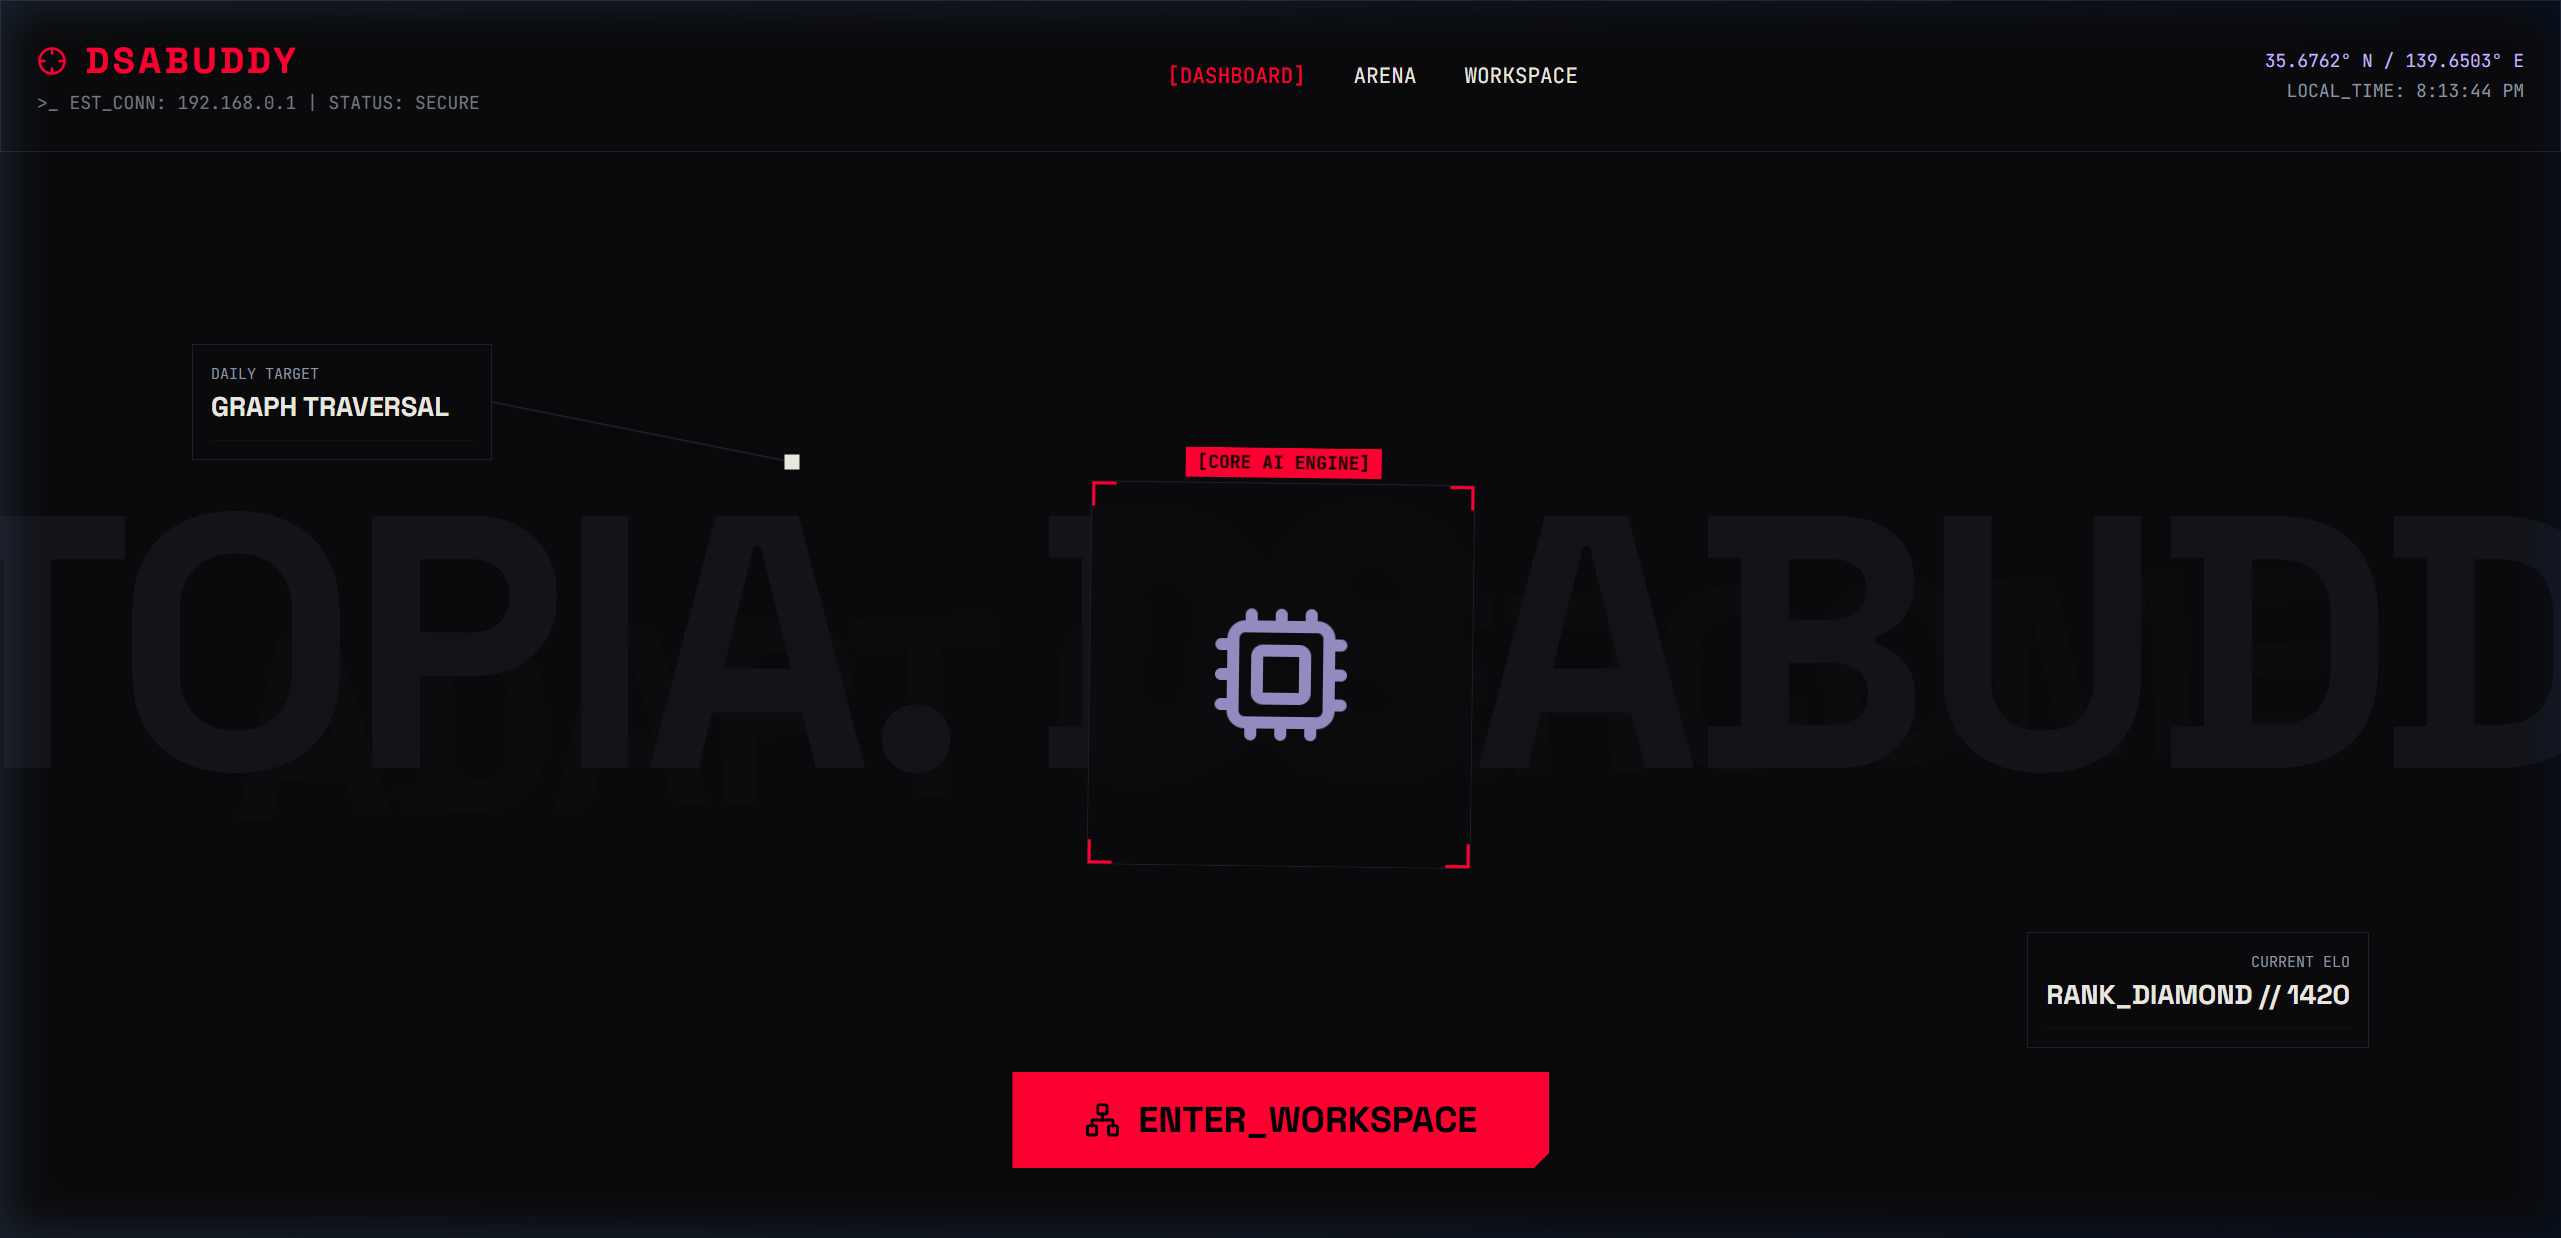
\includegraphics[width=0.7\textwidth]{screenshots/dashboard.png} \\
    \vspace{0.2cm}
    \caption{AI-driven insights and profile ELO tracking interface.}
\end{frame}

% ==========================================
% [8] VISUAL SHOWCASE: ARENA
% ==========================================
\begin{frame}{Visual Showcase: Real-Time Arena}
    \centering
    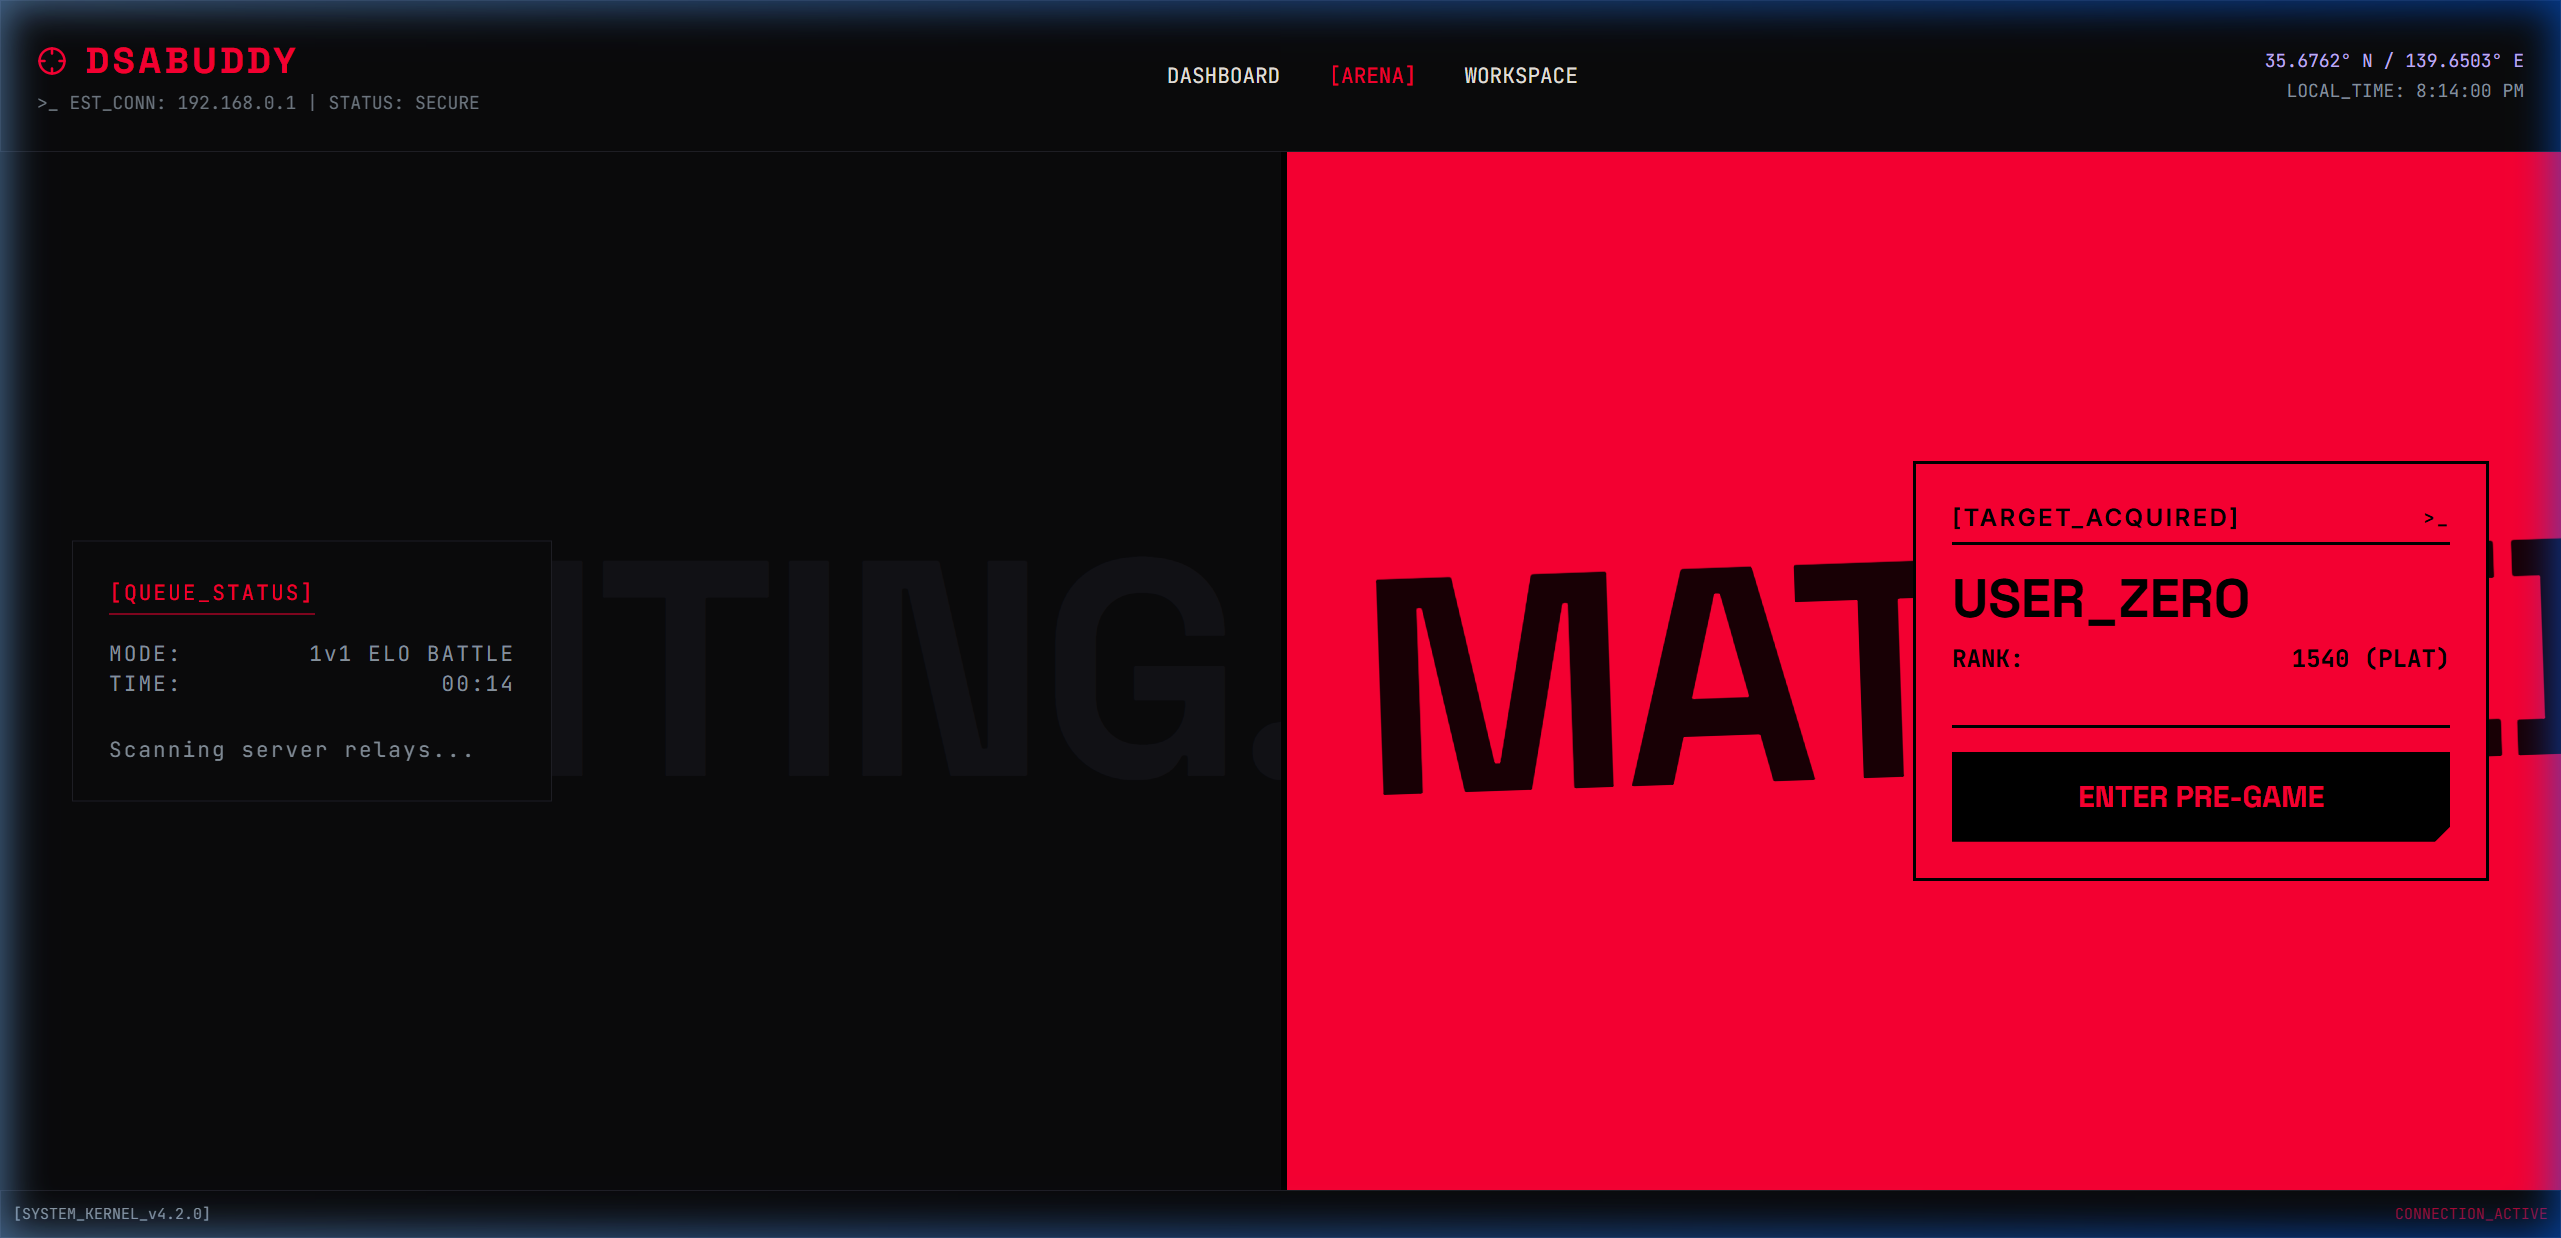
\includegraphics[width=0.7\textwidth]{screenshots/arena.png} \\
    \vspace{0.2cm}
    \caption{matchmaking lifecycle showing active topic queues.}
\end{frame}

% ==========================================
% [9] VISUAL SHOWCASE: WORKSPACE
% ==========================================
\begin{frame}{Visual Showcase: Workspace \& IDE}
    \centering
    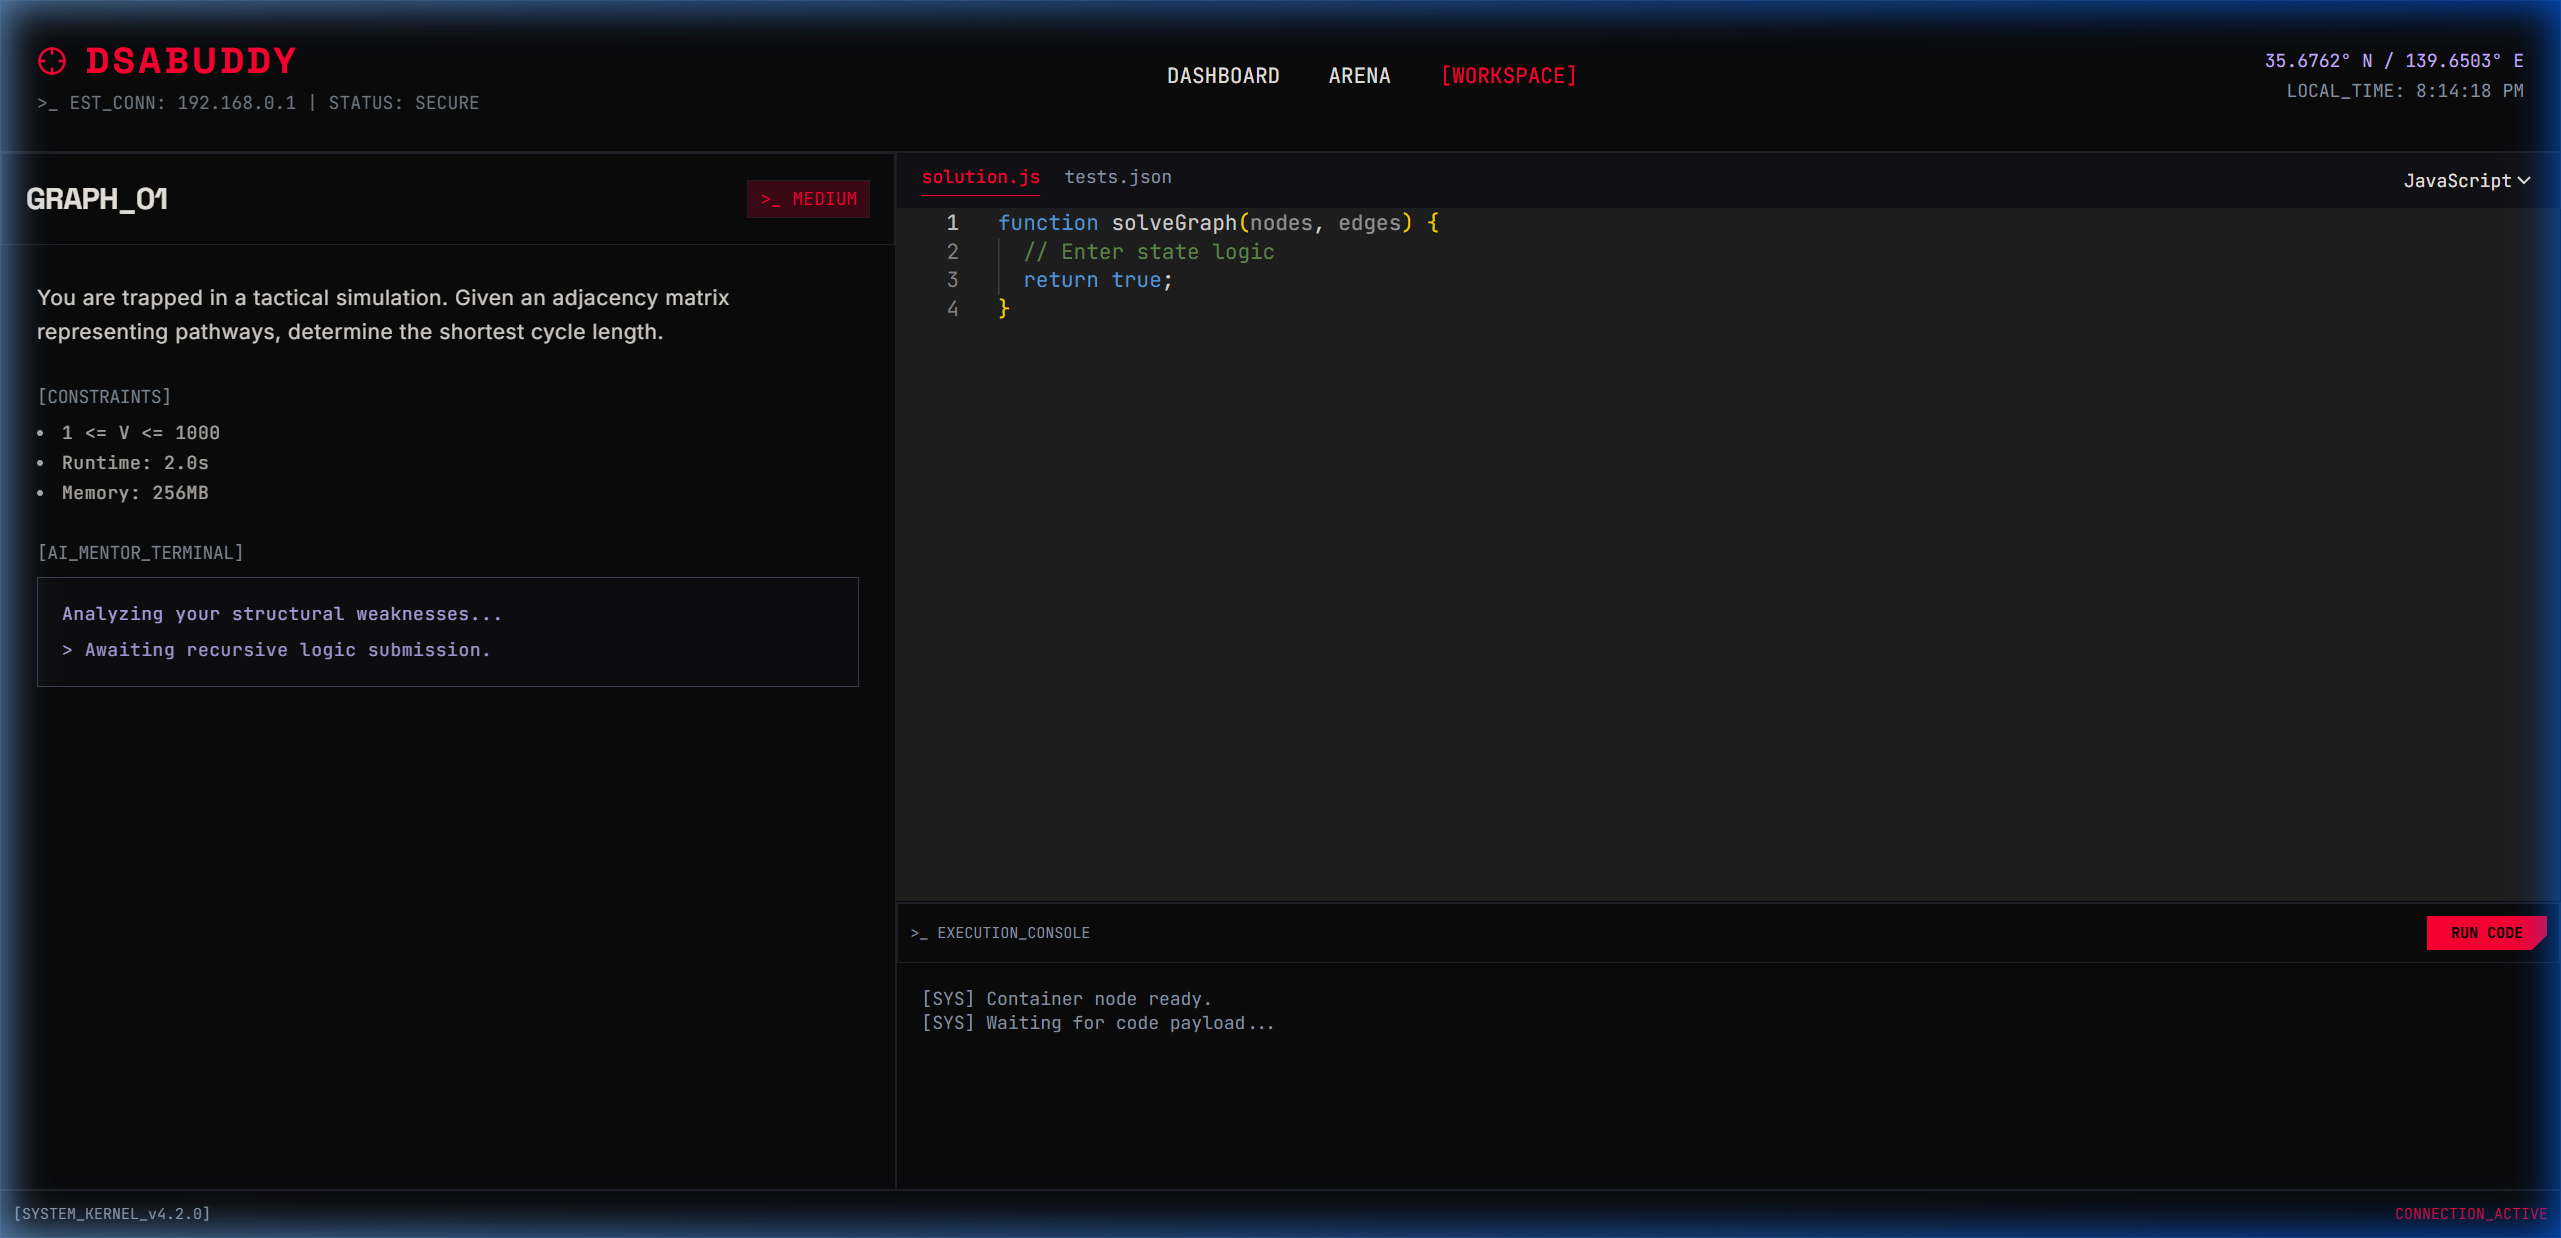
\includegraphics[width=0.7\textwidth]{screenshots/workspace.png} \\
    \vspace{0.2cm}
    \caption{Integrated Monaco Editor and AI Mentor feedback panel.}
\end{frame}

% ==========================================
% [10] IMPLEMENTATION PHASES
% ==========================================
\begin{frame}{Final Project Implementation Milestones}
    \begin{itemize}
        \item \textbf{Phase 1}: Core UI design and State management architecture.
        \item \textbf{Phase 2}: Backend WebSocket implementation and database integration.
        \item \textbf{Phase 3}: Matchmaking lifecycle optimization and Redis logic.
        \item \textbf{Phase 4}: AI Mentor integration and secure hint generation engine.
        \item \textbf{Final System}: Full-stack integration with end-to-end matchmaking loop.
    \end{itemize}
\end{frame}

% ==========================================
% [11] CONCLUSION
% ==========================================
\begin{frame}{Conclusion: The Future of DSA Training}
    \centering
    \Large \textbf{DSADojo Final System} \\
    \vspace{0.5cm}
    \normalsize
    \begin{itemize}
        \item Successfully transformed solo-practice into an engaging competitive platform.
        \item Built a scalable infrastructure for real-time pedagogical feedback.
        \item Proved that immersive UI/UX significantly improves user session duration.
    \end{itemize}
    \vspace{1cm}
    \textbf{Elite Practice. Tactical Logic. Mission Complete.}
\end{frame}

\end{document}
